% !TeX spellcheck = en_US
% !TeX root = ../build/users-fees.tex
% !TeX TXS-program:compile = txs:///xelatex/[--shell-escape]



\section{Basic Ethereum Fee Schema}

Before explaining the user fee schema followed in the zkEVM, let us devote this section to explain how the basic Ethereum fee schema works. Recall that the \textbf{Gas} is a unit that accounts the resources used when processing a transaction. \textbf{At the time of sending a transaction}, users have to define two parameters that will determine the fee imposed on them:

\begin{enumerate}
\item \texttt{gasLimit}: This parameter represents the upper limit of gas units that a user authorizes for consumption during the transaction.

\item \texttt{gasPrice}: It refers to the amount of Wei a user is willing to pay per unit of gas for the transaction execution. Trying to be more concrete, there exists a dynamic market interaction between users and network nodes. In Ethereum ecosystem, if a user desires to expedite the processing of their transaction, they must adjust the \texttt{gasPrice} accordingly. Essentially, a higher \texttt{gasPrice} becomes an incentive for network nodes to prioritize the associated transaction.

\end{enumerate}

At the \textbf{start of the transaction processing}, the following
amount of Wei is subtracted from the source account balance:
\[
\texttt{gasLimit} \cdot \texttt{gasPrice}.
\]
Then, when the processing of the transaction is finished, if $\texttt{gasUsed} > \texttt{gasLimit}$, the transaction is reverted. Otherwise, the amount of Wei associated with the unused gas is refunded. The refunded amount of Wei that is added back to the source account is calculated as:
\[
\texttt{gasLimit} \cdot \texttt{gasPrice} - \texttt{gasUsed} \cdot \texttt{gasPrice}.
\]

For reasons that will arise at the last section of this document, it is important to observe that when the transaction is being processed, the balance of the source account during transaction processing differs from its state at the time of sending the transaction. More specifically, if the \texttt{BALANCE} opcode is invoked during the transaction processing, the output will be
\[
\texttt{initialBalance} - \texttt{gasLimit} \cdot \texttt{gasPrice},
\]
where \texttt{initialBalance} represents the balance of the source account before the execution of the transaction.






%%%%%%%%%%%%%%%%%%%%%%%%%%%%%%%%%%%%%%%%%%%%%%%%%%%%%%%%%%%%%%%%%%%%%%%%%%%%%%%%
\section{Generic User Fee Strategy of Layer 2 Solutions}

In general, Layer 2 solutions adopt a fee strategy wherein the L2 gas price is a percentage of the L1 gas price. This approach aligns with the goal of making transactions less costly for the user. Using this approach, we can define \texttt{L2GasPrice} as follows:
\[
\texttt{L2GasPrice} = \texttt{L1GasPrice} \cdot \texttt{L1GasPriceFactor}.
\]
where \texttt{L1GasPrice} denotes the network variable indicating the minimum gas price required to sign a transaction, and $0 < \texttt{L1GasPriceFactor} < 1$ defines the reduction factor. For example, let us suppose that Layer 1 is accepting transactions having a signed gas price of $20$ GWei, so $\texttt{L1GasPrice} = 20$ and that L2 gas price is reduced a $96\%$. Then:
\begin{gather*}
\texttt{L1GasPrice} = 20 \text{ GWei} \text{ and } \texttt{L1GasPriceFactor} = 0.04 \ (4\% \text{ of L1 } \texttt{gasPrice}) \\
\text{therefore, } \texttt{L2GasPrice} = 20 \text{ GWei} \cdot 0.04 =  0.8 \text{ GWei}
\end{gather*}

You can check the current fees at \url{https://l2fees.info}. However, this is not as easy as it may seem and there are additional aspects to consider:

\begin{enumerate}[a)]
\item The gas price on L1 is subject to fluctuations over time (See Figure \ref{fig:refresh-gas-prices}). How does the zkEVM transaction processing mechanism account for these variations?

\item As we have said before, when initiating a transaction on Layer 1, increasing the gas price can serve to prioritize transactions. How does the Layer 2 solution effectively manage these priorities?

\item The Gas schema on Layer 1 may not necessarily align with the actual resources expended by the Layer 2 solution. How does the L2 solution address and reconcile any discrepancies between the L1 gas schema and the real resource utilization on L2?

\end{enumerate}

\begin{figure}[H]
\centering
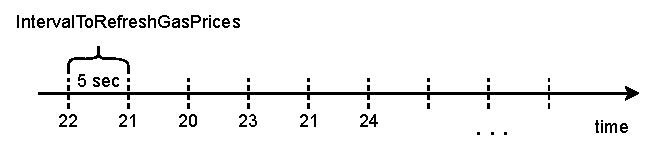
\includegraphics[width=0.8\columnwidth]{\zkevmdir/figures/architecture/economics-users-fees/l1-gasprice-refresh.drawio}
\caption{Observe that L1 gas prices, refreshed every $5$ seconds (which can be changed modifying a configuration parameter called \texttt{IntervalToRefreshGasPrices}) fluctuate over time.}
\label{fig:refresh-gas-prices}
\end{figure}

In the following sections, we will thoroughly examine the significance of fees in Layer 2 and provide detailed answers to the previously mentioned questions.

We will now delve into the initial phase of the process (see Figure \ref{fig:rpc}), which involves the \textbf{RPC} component of zkEVM. This phase spans from the moment the user submits the transaction, the price is estimated through a pre-execution of the transaction, to the final decision of storing it in the \textbf{Pool} or rejecting it based on a set of conditions.

\begin{figure}[H]
\centering
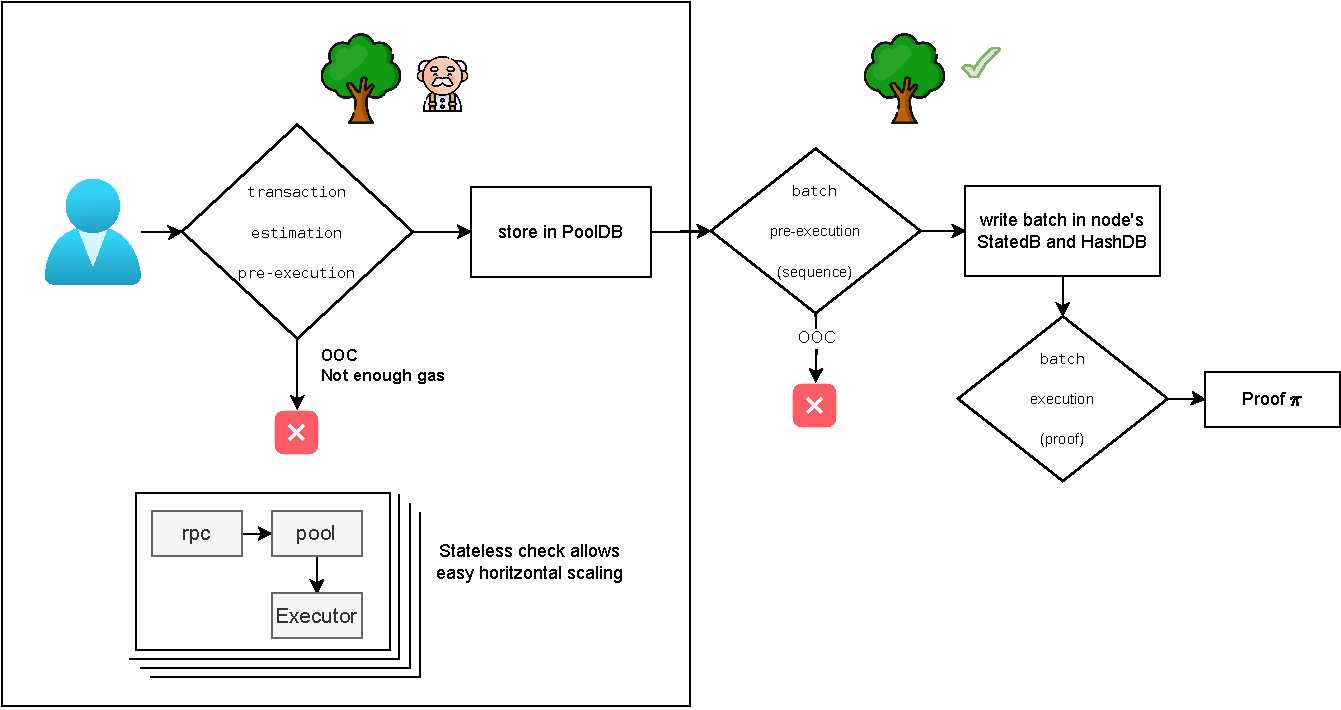
\includegraphics[width=0.8\columnwidth]{\zkevmdir/figures/architecture/economics-users-fees/rpc-preexecution.drawio}
\caption{Illustration of the first phase in the zkEVM flow, involving the \textbf{RPC} component, from user transaction submission to pre-execution to estimate optimal pricing and potential storage in the \textbf{Pool} or rejection.}
\label{fig:rpc}
\end{figure}







%%%%%%%%%%%%%%%%%%%%%%%%%%%%%%%%%%%%%%%%%%%%%%%%%%%%%%%%%%%%%%%%%%%%%%%%%%%%%%%%
\section{Gas Price Suggester}

This section will be devoted to constructing a scheme for the user to send a transaction to the zkEVM in such a way that their user experience is maximized. We will present different attempts, each addressing a problem from the previous one.

\subsection{Naive Approach}

Consider a scenario in which a user intends to send a transaction on Layer 2. However, the user lacks information regarding the appropriate gas price he/she has to sign with its transaction. Consequently, the user asks via RPC for a suggestion of the current gas price to sign with, as shown in Figure \ref{fig:suggest-l2-gas-price}. The suggested price will be \texttt{L2GasPrice}, which recall that is computed the following way:
\[
\texttt{L2GasPrice} = \texttt{L1GasPrice} \cdot \texttt{L1GasPriceFactor}.
\]
\begin{figure}[H]
\centering
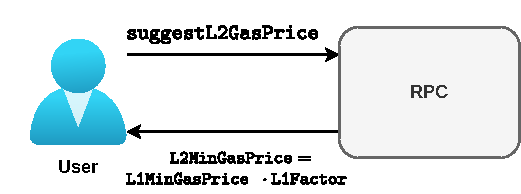
\includegraphics[scale=0.7]{\zkevmdir/figures/architecture/economics-users-fees/suggest-gasprice.drawio}
\caption{The user asks RPC for the suggested gas price.}
\label{fig:suggest-l2-gas-price}
\end{figure}

Now that the user knows a suggestion for the gas price he/she has to include, the user sends the desired L2 transaction with a choice of gas price that we will call \textbf{signed gas price}, denoted as \texttt{GasPriceSigned}. Observe that this choice can be  equal to, greater than, or lower than the suggested price, each resulting in distinct scenarios: either the acceptance or rejection of the transaction, as illustrated in Figure \ref{fig:send-tx}. We will delve on this later on.
\begin{figure}[H]
\centering
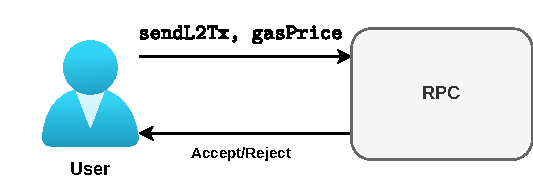
\includegraphics[scale=0.7]{\zkevmdir/figures/architecture/economics-users-fees/send-l2-tx-gasprice.drawio}
\caption{The user sends a transaction with the decided \texttt{GasPriceSigned} to RPC, a decision is taken on whether to accept or reject it.}
\label{fig:send-tx}
\end{figure}

In case the \texttt{GasPriceSigned} decided by the user is less than the current \texttt{L2GasPrice}, the transaction is automatically rejected and not included into the pool. This error is named \texttt{ErrGasPrice}.

\subsection{Decision Interval Approach}

\paragraph*{Problematic}

The previous framework has a limitation as there is a time gap between asking for a suggested gas price and sending the transaction in which the gas price can fluctuate. This fact leads the unwanted situation depicted in Figure \ref{fig:bad-ux}:
\begin{figure}[H]
\centering
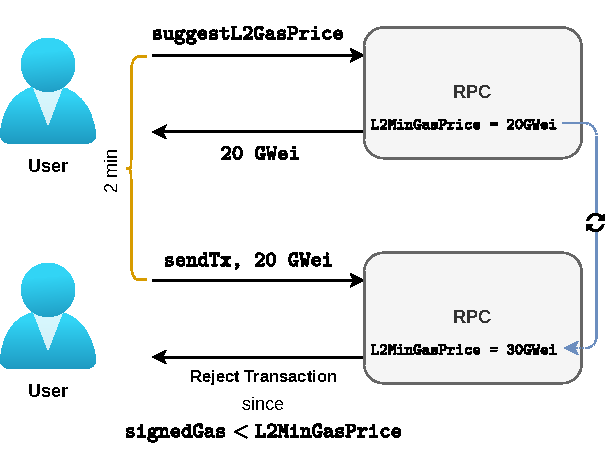
\includegraphics[scale=0.7]{\zkevmdir/figures/architecture/economics-users-fees/fees-bad-ux.drawio}
\caption{The user asks for a suggested price, the current suggested gas price is of $20$ GWei and decides to sign $20$ GWei, but when he sends the transaction the suggested gas price has increased to $30$ GWei and the transaction is rejected. }
\label{fig:bad-ux}
\end{figure}

In Figure \ref{fig:bad-ux} we can observe that although the user has sent a gas price according to the suggested price, after the time lapse between one step and the other, the price has increased and the transaction is rejected.

\paragraph*{Solution}

The \textbf{solution} is to give a user some period of time in order to make the choice and sending the transaction. More specifically, we give a margin of $5$ minutes (controlled by the \texttt{MinAllowedGasPriceInterval} parameter). The \texttt{MinL2GasPrice} is defined as the minumum suggested gas price of $5$ minutes before sending the transaction refreshed every $5$ seconds (controlled by the \texttt{IntervalToRefreshGasPrices} parameter). If the signed gas price does not strictly exceed \texttt{MinL2GasPrice},
\[
\texttt{GasPriceSigned} > \texttt{L2MinGasPrice},
\]
we automatically \textbf{reject} the transaction, since it will not be possible to cover costs. Figure \ref{fig:minimum-gas-price} depicts an example on how \texttt{MinL2GasPrice} is computed, which in this precise case is $18$ GWei.

\begin{figure}[H]
\centering
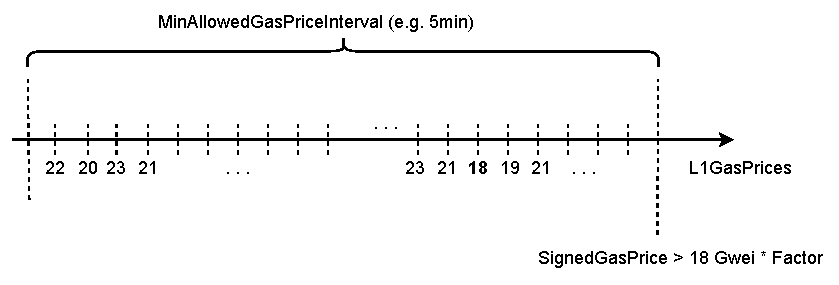
\includegraphics[scale=0.7]{\zkevmdir/figures/architecture/economics-users-fees/min-allowed-price-interval.drawio}
\caption{Timeline displaying the current \texttt{L1GasPrice} and its associated suggested gas price. In this case \texttt{MinL2GasPrice}=$18$. }
\label{fig:minimum-gas-price}
\end{figure}

This previous parameters can be configured in the Polygon zkEVM node configuration files. More specifically, it can be configures in the \texttt{[Pool]} section of the configuration TOML, which can be found \href{https://github.com/0xPolygonHermez/zkevm-node/blob/b938572f138ba6cc40ef6736153c469afeb11c96/config/default.go#L37}{here}.

\vspace{1em}

\begin{toml}
[Pool]
...
DefaultMinGasPriceAllowed = 0
MinAllowedGasPriceInterval = "5m"
PollMinAllowedGasPriceInterval = "1s"
IntervalToRefreshGasPrices = "5s"
...
\end{toml}

%TODO Marc: Review and extend.
%Where the meaning of the parameters is:
%
%\begin{itemize}
%\item \texttt{DefaultMinGasPriceAllowed:} It is the default min gas price to suggest.
%\item \texttt{MinAllowedGasPriceInterval:} It is the interval to look back of the suggested min gas price for a transaction.
%\item \texttt{PollMinAllowedGasPriceInterval:} It is the interval to poll L1 to find the suggested L2 min gas price.
%\item \texttt{IntervalToRefreshGasPrices:} It is the interval to refresh L2 gas prices.
%\end{itemize}
%
%When computing the L1 \texttt{gasPrice}, we can activate the \texttt{multigasprovider}, which allows using multiples sources for computing the L1 \texttt{gasPrice}:
%\begin{toml}
%[Etherman]
%...MultiGasProvider = false
%\end{toml}
%
%\vspace{10 mm}


\subsection{Final Approach}

\paragraph*{Problematic}

However, in the previous design, the zkEVM endpoint responsible for offering a gas price suggestion to the user, known as \textbf{L2 Gas Price Suggester}, faces a significant problem design. The price of posting transactional data to L1 is charged to the zkEVM network to the \textbf{full L1 price}. Therefore, if we propose a gas price using \texttt{L1GasPriceFactor}, representing the measure of computational reduction in L2, there is a risk of running out of Wei reserves for posting data to L1.

\paragraph*{Solution}

In order to solve the previous situation, we will recommend a slightly higher percentage of the gas price to the user, employing a \texttt{SuggesterFactor} of $0.15 \approx 4 \cdot \texttt{L1GasPriceFactor}$:
\[
\texttt{GasPriceSuggested} = \texttt{L1GasPrice} \cdot \texttt{SuggestedFactor}.
\]


\subsection{Numerical Example: \texttt{L2MinGasPrice}}


In Figure \ref{fig:numerical-example} we can observe that when the user queries the suggested gas price through the RPC, the network responds the current suggested gas price computed as $0.15 \cdot 19 = 2.85$, where $19$ is the current L1 gas price, updated every $5$ seconds. Observe that, using the naive approach, the user should have signed for a gas price strictly higher than $3.15$, since the L1 gas price at the moment of sending the transaction is $21$. However, using the final approach, at the time of sending the transaction, the RPC will accept the transaction as long as $\texttt{GasPriceSigned}$ is strictly higher than the minimum suggested gas price from the 5 minutes interval (highlighted in \textbf{bold} in the figure), which in this instance is $19 \cdot 0.15 = 2.85$. In order to get his transaction accepted, the user sets the gas price of the transaction to $\texttt{GasPriceSigned} = 3.3 > 2.85 = \texttt{L2MinGasPrice}.$ The user has signed at a higher gas price than the suggested to ensure that the transaction is executed and maybe prioritize it among others.


\begin{figure}[H]
\centering
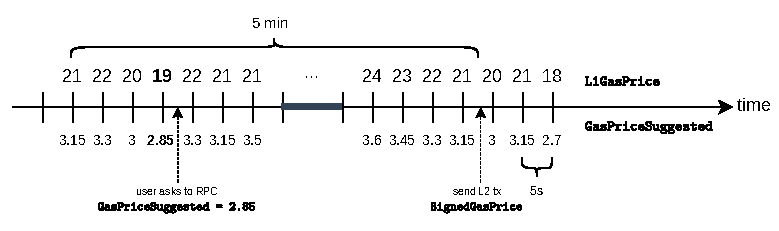
\includegraphics[scale=1]{\zkevmdir/figures/architecture/economics-users-fees/example-minimum-gas-price.drawio}
\caption{The user asks for a \texttt{GasPriceSuggested} = $2.85$ and decides to set \texttt{SignedGasPrice} = $3.3$ to ensure that the transaction is executed.}
\label{fig:numerical-example}
\end{figure}





%%%%%%%%%%%%%%%%%%%%%%%%%%%%%%%%%%%%%%%%%%%%%%%%%%%%%%%%%%%%%%%%%%%%%%%%%%%%%%%%
\section{Dealing with L1/L2 Cost Discrepancies}

\subsection{Cost Discrepancies Challenges}

As we have said before, in Ethereum, \textbf{gas} accounts for the resources used by a transaction. In particular, it takes into account two elements in particular: the \textbf{data availability}, that is, the transactions bytes and the \textbf{processing resources}, like CPU, Memory and Storage. A notable challenge arises when certain operations consume low gas in Layer 1 but represent a major cost in Layer 2. In other words, the reduction factor expressed in the L1-L2 gas price relationship
\[
\texttt{L2GasPrice} = \texttt{L1GasPrice} \cdot \texttt{L1GasPriceFactor}
\]
may not be constant among all the computational resources, introducing a problem.

L2 execution costs are variable, depending on the state of the transaction and typically offer a smaller cost per gas. However, the costs associated with data availability are fixed once the transaction is known, and they are directly proportional to L1 data availability costs. Consequently, in our pricing schema, L2 transactions with high data availability costs and small execution costs are a significant challenge. This presents another pricing misalignment issue we need to face.

\subsection{Possible Solutions}

Recall that the Ethereum fee in L1 is computed as
\[
\texttt{gasUsed} \cdot \texttt{gasPrice},
\]
giving us two ways of solving the misalignment problem between costs in L1 and L2:

\begin{enumerate}[(A)]
\item \textbf{Arbitrum Approach. Increase \texttt{gasUsed}. }
This approach involves modifying the gas schema to elevate the Gas costs associated with data availability. While this strategy is relatively straightforward to implement and comprehend, it comes with a notable implication: \textbf{it changes the Ethereum protocol}. An L1 Ethereum transaction may execute different when compared to the same transaction executed in L2.

\item \textbf{Effective Gas Price Approach. Increase \texttt{gasPrice}. }
If we aim to avoid modifying the gas, the alternative is to increase the gas price to cover the costs. Unlike the previous approach, this doesn't alter the Ethereum specifications. However, determining a fair gas price becomes a complex task. Moreover, we have to take into account that L2 users should be able to prioritize its transactions also increasing gas price, as they are used to. \textbf{This is actually our approach.}
\end{enumerate}


\subsection{Effective Gas Price Approach}

We will now develop how the \textbf{Effective Gas Price Approach} works. First, the user signs a relatively high gas price at the time of sending the L2 transaction. Later on, by pre-executing the sent transaction, the \textbf{sequencer} establishes a fair gas price according to the amount of resources used. To do so, the \textbf{sequencer} provides an \texttt{EffectivePercentage}, which represents the portion of the total charged to the user. In other words, this percentage will be used in order to compute the factor of the signed transaction's signed gas price which should be refunded to the user.

To calculate the \texttt{EffectivePercentage}, one option is to consider the pricing resources based on the number of \textbf{consumed counters} within our proving system. However, understanding this metric can be challenging for users because stating the efficiency through counters is not intuitive at the time of prioritizing their transactions. As we want to prioritize a positive user experience, we will consider an alternative where gas is used for calculations, as it is more user-friendly. So, our primary objective is to compute \texttt{EffectivePercentage} exclusively using gas, allowing users to prioritize their transactions through the use of gas price without the need for intricate counter-based considerations. The effective percentage is computes as follows:
\[
\texttt{EffectivePercentage} = \frac{\texttt{GasPriceFinal}}{\texttt{GasPriceSigned}}.
\]
Observe that, by modifying \texttt{GasPriceFinal}, which is the gas price charged at the end of the whole processing by the sequencer, we can modify the amount of Wei that we will charge to the user in order to process the sent transaction.

To send this percentage, the \textbf{sequencer} provides a single byte \texttt{EffectivePercentageByte} $\in \{0, 1, \dots, 255 \}$, which is computed from the \texttt{EffectivePercentage}:
%TODO: Review this formula
\[
\texttt{EffectivePercentageByte} = (\texttt{EffectivePercentage}\cdot 256) - 1.
\]

As having \texttt{EffectivePercentage} implies having \texttt{EffectivePercentageByte}, and vice versa, we will abuse of notation and use them interchangeably as \texttt{EffectivePercentage}. For example, setting an \texttt{EffectivePercentageByte} of $255 (= \texttt{0xFF})$ would mean that the \texttt{EffectivePercentage} = $1$ so user would pay the totality of the gas price signed when sending the transaction:
\[
\texttt{GasPriceFinal} = \texttt{GasPriceSigned}.
\]

In contrast, setting \texttt{EffectivePercentageByte} to $127$ would mean that
\[
\texttt{EffectivePercentage} = 0.5
\]
so it will reduce the gas price signed by the user to the half:
\[
\texttt{GasPriceFinal} = \frac{\texttt{GasPriceSigned}}{2}.
\]
This implies that the user will be refunded half of the price he initially signed for. Observe that, in this schema, users \textbf{must trust the sequencer}.





%%%%%%%%%%%%%%%%%%%%%%%%%%%%%%%%%%%%%%%%%%%%%%%%%%%%%%%%%%%%%%%%%%%%%%%%%%%%%%%%
\section{Introducing \texttt{BreakEvenGasPrice}}

As service providers, our primary goal is to \textbf{avoid accepting transactions that result in financial losses}. To attain this objective, we will determine the \texttt{BreakEvenGasPrice}, representing the lowest gas price at which we do not incur losses. As explained before, we will split the computation in two to take into account differently costs associated with data availability and costs associated with processing resources.
%TODO he canviat el final de la frase q posava: costs associated with used gas


\subsection{Costs Associated with Data Availability}

Costs associated with Data Availability will be computed as
\[
\texttt{DataCost} \cdot \texttt{L1GasPrice},
\]
where \texttt{DataCost} is the cost in Gas for data in L1.

In the Ethereum ecosystem, the cost of data varies depending on whether it involves zero bytes or non-zero bytes. In particular, \textbf{non-zero bytes} cost \textbf{$16$ Gas} meanwhile \textbf{zero bytes} \textbf{$4$ Gas}. Also recall that, when computing non-zero bytes cost we should take into account some constant data always appearing in a transaction and are not included in the RLP: the signature, consisting on $65$ bytes and the previously defined \texttt{EffectivePercentageByte}, which consists in a single byte. This results in a total of $66$ constantly present bytes.

Taking all in consideration, \texttt{DataCost} can be computed as:
\begin{gather*}
\texttt{DataCost} = \underbrace{(\texttt{TxConstBytes} + \texttt{TxNonZeroBytes}) \cdot \texttt{NonZeroByteGasCost}}_\text{Non Zero Bytes} \\
+ \underbrace{\texttt{TxZeroBytes} \cdot \texttt{ZeroByteGasCost}}_\text{Zero Bytes}
\end{gather*}
where \texttt{TxZeroBytes} (respectively \texttt{TxNonZeroBytes}) represents the count of zero bytes (respectively non-zero bytes) in the raw transaction sent by the user.


\subsection{Computational Costs}

For the computational cost, we will use the following formula:
\[
\texttt{GasUsed} \cdot \texttt{L2GasPrice},
\]
where recall that we can obtain \texttt{L2GasPrice} by multiplying \texttt{L1GasPrice} by chosen factor less than $1$
\[
\texttt{L2GasPrice} = \texttt{L1GasPrice} \cdot \texttt{L1GasPriceFactor}.
\]
In particular, we will choose a factor of $0.04$.

In contrast to data availability costs, to compute computational costs we will need to \textbf{execute} the transaction.

\subsection{Total Price of the Transaction}

Combining both \textbf{data} and \textbf{computational} costs, we will refer to it as \texttt{TotalTxPrice}:
\[
\texttt{TotalTxPrice} = \underbrace{\texttt{DataCost} \cdot \texttt{L1GasPrice}}_\text{Data availability cost} + \underbrace{\texttt{GasUsed} \cdot \texttt{L1GasPrice} \cdot \texttt{L1GasPriceFactor}}_\text{Computational cost}
\]

To establish the gas price at which the total transaction cost is covered we can compute \texttt{BreakEvenGasPrice} as the following ratio:
\[
\texttt{BreakEvenGasPrice} = \frac{\texttt{TotalTxPrice}}{\texttt{GasUsed}}.
\]
Additionally, we incorporate a factor $\texttt{NetProfit} \geq 1$ that allows us to achieve a slight profit margin:
\[
\texttt{BreakEvenGasPrice} = \frac{\texttt{TotalTxPrice}}{\texttt{GasUsed}} \cdot \texttt{NetProfit}.
\]

We could now conclude that if
\[
\texttt{SignedGasPrice} > \texttt{BreakEvenGasPrice}
\]
it is supposed to be financially safe to accept the transaction. But at this point the following problem arises: in the RPC component, we're only pre-executing the transaction, meaning we're using an incorrect state root. Consequently, the \texttt{GasUsed} is only an approximation. This implies that we need to multiply the result by a chosen factor before comparing it to the signed price. This ensures that the costs are covered in case more gas is ultimately required to execute the transaction. This factor is named \texttt{BreakEvenFactor}. Now we can conclude that if:
\[
\texttt{SignedGasPrice} > \texttt{BreakEvenGasPrice} \cdot \texttt{BreakEvenFactor}
\]
it is safe to accept the transaction.

Observe that we still need to introduce gas price prioritization, which will be covered later on.


\subsection{Numerical Example: Computing \texttt{BreakEvenGasPrice}}

Recall the example proposed before, where the \texttt{GasPriceSuggested} provided by RPC was $2.85$ GWei/Gas but the user ended up by setting \texttt{GasPriceSigned} to $3.3$. Figure \ref{fig:numerical-example-break-even-gas-price} depicts the current situation.

\begin{figure}[H]
\centering
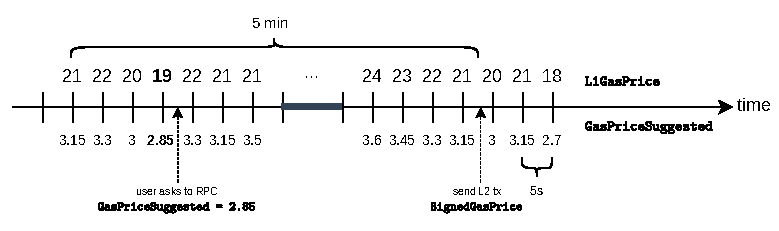
\includegraphics[scale=0.9]{\zkevmdir/figures/architecture/economics-users-fees/example-minimum-gas-price.drawio}
\caption{Timeline displaying the current \texttt{L1GasPrice} and its associated suggested gas price.}
\label{fig:numerical-example-break-even-gas-price}
\end{figure}

Suppose the user sends a transaction having: $200$ non-zero bytes, including the constant ones and $100$ zero bytes. Moreover, at the time of pre-executing the transaction, which is done without getting an \textbf{OOC} error, $60,000$ Gas is consumed. Recall that, since we are using a \textbf{wrong} state root, this gas is only an estimation. Hence, following the formulas previously explained, the total transaction cost is of
\begin{gather*}
\texttt{TotalTxPrice} = \texttt{DataCost} \cdot \texttt{L1GasPrice} + \texttt{GasUsed} \cdot \texttt{L1GasPrice} \cdot \texttt{L1GasPriceFactor} \Rightarrow \\
\texttt{TotalTxPrice} = \left( 200 \cdot 16 + 100 \cdot 4 \right) \cdot 21 + 60,000 \cdot 21 \cdot 0.04 = 126,000 \text{ GWei}.
\end{gather*}

Observe that $21$ appearing in the substitution is the \texttt{L1GasPrice} at the time of sending the transaction.

Now, we are able to compute the \texttt{BreakEvenGasPrice} as
\[
\texttt{BreakEvenGasPrice} = \frac{\texttt{TotalTxPrice}}{\texttt{GasUsed}} = \frac{126,000 \text{ GWei}}{60,000 \text{ Gas}} \cdot 1,2 = 2.52 \text{ GWei/Gas}.
\]

We have introduced a \texttt{NetProfit} value of $1.2$, indicating a target of a $20\%$ gain in this process. At a first glance, we might conclude acceptance since $\texttt{GasPriceSigned} = 3.3 > 2.52$ but, recall that this is only an estimation, gas consumed with the correct state root can differ. To avoid this issue, we introduce a \texttt{BreakEvenFactor} of $30\%$ to account for estimation uncertainties:
\[
\texttt{GasPriceSigned} = 3.3 > 3.276 = 2.52 \cdot 1.3 = \texttt{BreakEvenGasPrice} \cdot \texttt{BreakEvenFactor}.
\]

Consequently, we decide to \textbf{accept the transaction}.


\subsection{Numerical Example: Importance of \texttt{BreakEvenFactor}}

Imagine we disable the \texttt{BreakEvenFactor} setting it to $1$. Our original transaction's pre-execution consumed $60,000$ Gas
\[
\texttt{GasUsedRPC} = 60,000.
\]

However, imagine that the correct execution at the time of sequencing consumes $35,000$ Gas. If we recompute \texttt{BreakEvenGasPrice} using this updated used gas, we get $3.6 \text{GWei/Gas}$, which is way higher than the original one. That means that, we should have charged the user with a higher gas price in order to cover the whole transaction cost, which now is of $105,000$ GWei.

But, since we are accepting all the transactions signing more than $2.85$ of gas price, we do not have margin to increase more. In the worst case we are loosing
\[
105,000 - 35,000 \cdot 2.85 = 5,250 \text{ GWei}.
\]

Introducing \texttt{BreakEvenFactor} we are limiting the accepted transactions to the ones having
\[
\texttt{GasPriceSigned} \geq 3.27,
\]
in order to compensate such losses.

In this case, we have the flexibility to avoid losses and adjust both user and our benefits since
\[
105,000 - 35,000 \cdot 3.27 < 0.
\]

\paragraph*{Final Note}
In the example, even though we assumed that the decrease in \texttt{BreakEvenGasPrice} is a result of executing with a correct state root, it can also decrease significantly due to a substantial reduction in \texttt{L1GasPrice}.





\section{\texttt{EffectiveGasPrice}: Introducing Priority}

Prioritization of transactions in Ethereum is determined by \texttt{GasPriceSigned}: transactions signed at a higher price will be given priority. To implement this, consider that users are only aware of two gas price values: the one signed with the transaction, called \texttt{GasPriceSigned} and the current \texttt{GasPriceSuggested}, which is the one that provides the RPC. 

It is important to note that this part of the process \textbf{is not} computed in the \textbf{RPC} but in the \textbf{Sequencer}, so it possible that the suggested gas price at this moment differs from the suggested one when user sent the transaction.

At the time of sequencing a transaction, we should prioritize ones among the others, depending basically on both \texttt{GasPriceSigned} and current \texttt{GasPriceSuggested}. In the case that $\texttt{GasPriceSigned} > \texttt{GasPriceSuggested}$, we establish a priority ratio as follows:
\[
\texttt{PriorityRatio} = \frac{\texttt{GasPriceSigned}}{\texttt{GasPriceSuggested}} - 1.
\]

If $\texttt{GasPriceSigned} \leq \texttt{GasPriceSuggested}$, the user has chosen not to prioritize its transaction, and maybe we can reject the transaction due to low gas price. In this case, we establish a priority ratio to be $0$.

Finally, the \texttt{EffectiveGasPrice} will be computed as:
\[
\texttt{EffectiveGasPrice} = \texttt{BreakEvenGasPrice} \cdot (1 + \texttt{PriorityRatio}).
\]


\subsection{Numerical Example: Priority}

 Let's see it with an example. Recall that, in the previous example, we were signing a gas price of $3.3$ at the time of sending the transaction. Suppose that, at the time of sequencing a transaction, the suggested gas price is 3:
\[
\texttt{GasPriceSigned} = 3.3, \quad \texttt{GasPriceSuggested} = 3.
\]
The difference between both is taken into account in the priority ratio:
\[
\texttt{PriorityRatio} = \frac{3.3}{3} - 1 = 0.1.
\]
Henceforth, the estimated \texttt{EffectiveGasPrice} (that is, the one using the RPC gas usage estimations) will be
\[
\texttt{EffectiveGasPrice} = 2.52 \cdot (1 + 0.1) = 2.772 \text{ GWei/Gas}.
\]
